\documentclass{article} 

\usepackage{amsmath,amsthm}     
\usepackage{graphicx}     
\usepackage{hyperref} 
\usepackage{url}
\usepackage{amsfonts} 
\usepackage[margin=0.7in]{geometry}
\usepackage{float}
\usepackage{multicol, multirow}
\usepackage{arydshln}
\usepackage{subcaption}
\usepackage[french]{babel}



\allowdisplaybreaks

\makeatletter
\@addtoreset{footnote}{page}
\makeatother

%%%%%%%%%%%%%%%%%%%%%%%%%%%%%%%%%%%%%%%%%%%%%%%%%%
\begin{document}


\title{BIML GNN : Prédiction de lien \\
\footnotesize{VGAE et autre joyeusetés}}
\author{Bonhoure Timothé, Martinez Christophe}                      %%%% your final manuscript.

\maketitle
\tableofcontents
\section*{Abstract}
\newpage

\section{Méthode}

Dans le cadre de ce projet, nous avons décidé de développer notre propre décodeur pour la prédiction de liens. Ce décodeur est composé de deux couches linéaires séparées par une fonction d'activation ReLU. Pour évaluer son efficacité, nous avons mis en place deux modèles :
\begin{itemize}
    \item Un VGAE (Variational Graph Autoencoder) avec un encodeur composé d'une couche GCNConv suivie de deux couches GCNConv pour encoder la moyenne et l'écart type dans l'espace latent.
    \item Un GAE (Graph Autoencoder) composé d'une seule couche GCNConv.
\end{itemize}
Pour la préparation des données nous utilisons la méthode suivante :
\begin{verbatim}
torch_geometric.transforms.RandomLinkSplit(is_undirected=True, split_labels=True, num_val=0)
\end{verbatim}
Cette méthode nous permet de générer des jeux d’entraînement et de test de liens existants dans les données d'origine (liens positifs) et non existants dans les données d'origine (liens négatifs). Elle nous permet aussi de définir que ces liens sont non orientés et que donc pour chaque paire d’indices formant le lien, le premier indice est inférieur au deuxième.
Nous avons opté pour l'utilisation de l'optimiseur Adam avec un taux d'apprentissage de 0,01 et un terme de régularisation (\texttt{weight\_decay}) de \(5e^{-4}\).
Tout les modèles présent auront une taille de sortie de l'espace latent de 32.

Dans l'ensemble de nos expérimentations, nous fournissons aux modèles de prédiction des données comprenant la latitude, la longitude et le pays (converti en un code numérique). En plus de cela, nous avons décidé d'explorer l'ajout de l'information sur le degré de chaque nœud et de comparer les résultats.
Les degrés des nœuds sont déterminés en utilisant notre connaissance du graphe réel. Cependant, lorsque nous envisageons d'intégrer un nouvel aéroport à notre base de données, il devient envisageable d'estimer le degré potentiel du nœud associé à cet aéroport en se basant sur les flux d'arrivées et de départs des avions de cet aéroport. Ainsi, la réalisation de ce test nous semble pertinente et justifiée.


\section{Étude du dropout}
Nous avons essayé d'améliorer le modèle VGAE en y incorporant une couche de dropout entre la première et la deuxième couche. 
Nous avons laissé la valeur de dropout à la valeur par défaut soit 0.5. 
Les modèles ont été entraîné sur 2000 epochs. 
Ce processus a été répété 60 fois pour obtenir des statistiques sur l'apprentissage.
Le processus a été réalisé à la fois dans la situation ou le degré est inconnu et dans la situation ou il est connu

\subsection{Résultats}
Les résultats au bout des 2000 epochs ont été compilé dans le tableau \ref{tab:dropout}.
L'évolution au cour de l'apprentissage de l'AUC et la précision moyenne ont elle été représenté sur la figure \ref{fig:dropout}.
Les résultats montre sans équivoque que la présence de cette couche réduit énormément les performances du modèles sans réduire de manière suffisante l'écart type et cela dans les deux situations.
En effet en regardant les courbes de la figure \ref{fig:dropout} on remarque que seul les instances les plus performantes de VGAE avec du dropout arrive à dépasser la médiane des instances de VGAE sans dropout.
Pour la suite des tentatives on ne conserverat donc pas le dropout.

\begin{table}[H]
    \centering
    \captionsetup{justification=centering}
    \begin{tabular}{|c|*{2}{c:c:c|}} 
        \hline
        \multirow{2}{*}{modèle} &\multicolumn{3}{|c|}{Sans Degrée} & \multicolumn{3}{|c|}{Avec Degrée} \\
        \cline{2-7}
        & \footnotesize{AUC} & \footnotesize{AP} & \footnotesize{temps} &\footnotesize{AUC} & \footnotesize{AP} & \footnotesize{temps} \\
        \hline
        VGAE              & \textbf{.823}(\textbf{.015}) & \textbf{75.6\%}(2.2\%) & \textbf{107.8s}(\textbf{4.9s}) & .830(.023) & 75.5\%(2.8\%) & 110.9s(6.2s)\\
        VGAE with dropout & .785(.017)                   & 70.6\%(\textbf{1.9\%}) & 109.3s(5.3s) & .781(.021)      & 70.0\%(2.6\%) & 112.0s(9.345)\\
        \hline
    \end{tabular}
    \caption{Résultats de l'utilisation du dropout. \\ \footnotesize Dans chaque case est indiqué la moyenne et l'écart-type au format : moyenne(écart-type)}
    \label{tab:dropout}
\end{table}
\begin{figure}[H]
    \centering
    \captionsetup{justification=centering}
    \begin{subfigure}{0.45\textwidth}
      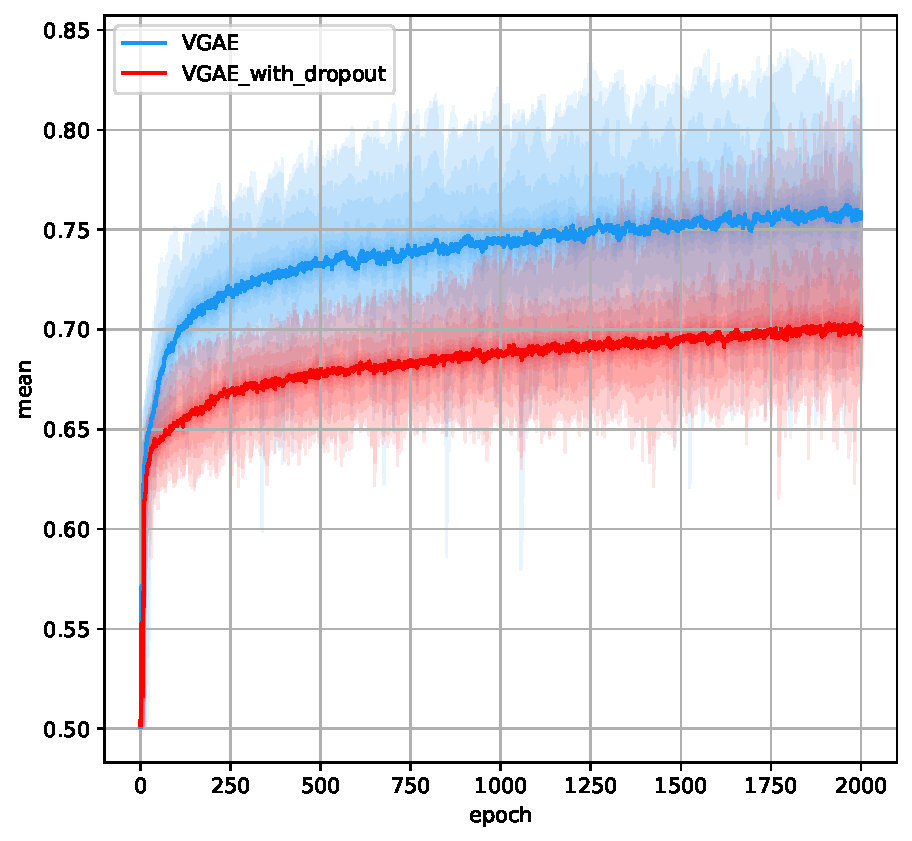
\includegraphics[width=\textwidth]{graphics/APs_degree_dropout_cinf.svg.pdf}
      \centering
      \caption{précision moyenne au cours de l'apprentissage\\ avec l'information de degrée}
    \end{subfigure}
    \begin{subfigure}{0.45\textwidth}
      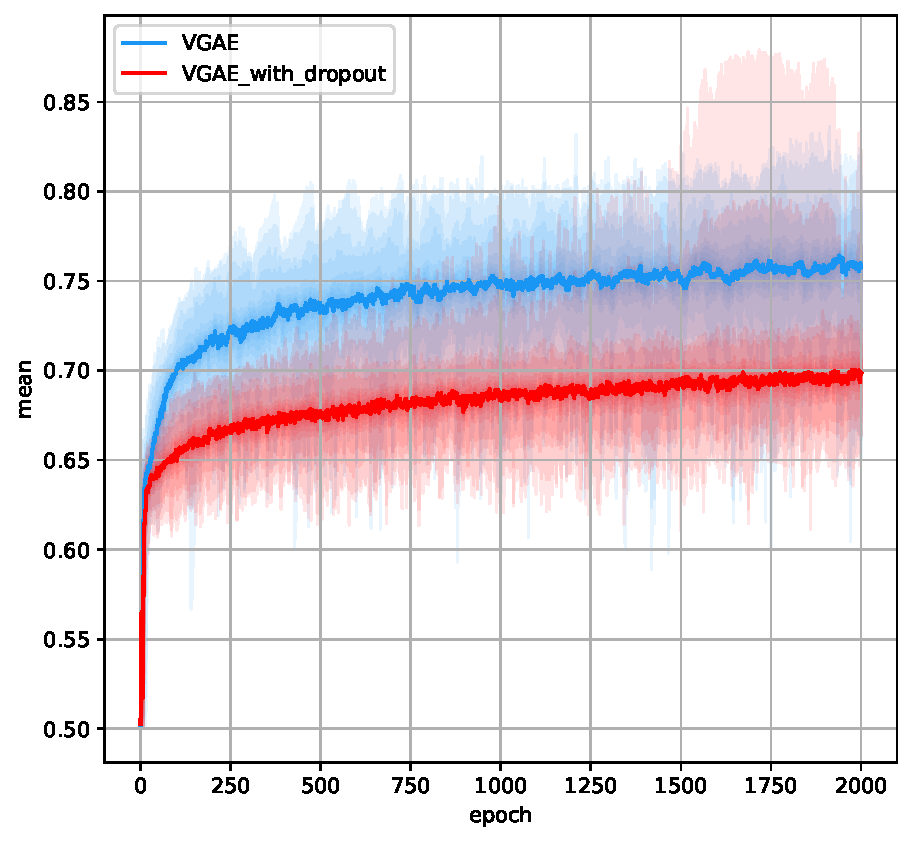
\includegraphics[width=\textwidth]{graphics/APs_no_degree_dropout_cinf.svg.pdf}
      \centering
      \caption{précision moyenne au cours de l'apprentissage\\ sans l'information de degrée}
    \end{subfigure}
    
    \begin{subfigure}{0.45\textwidth}
      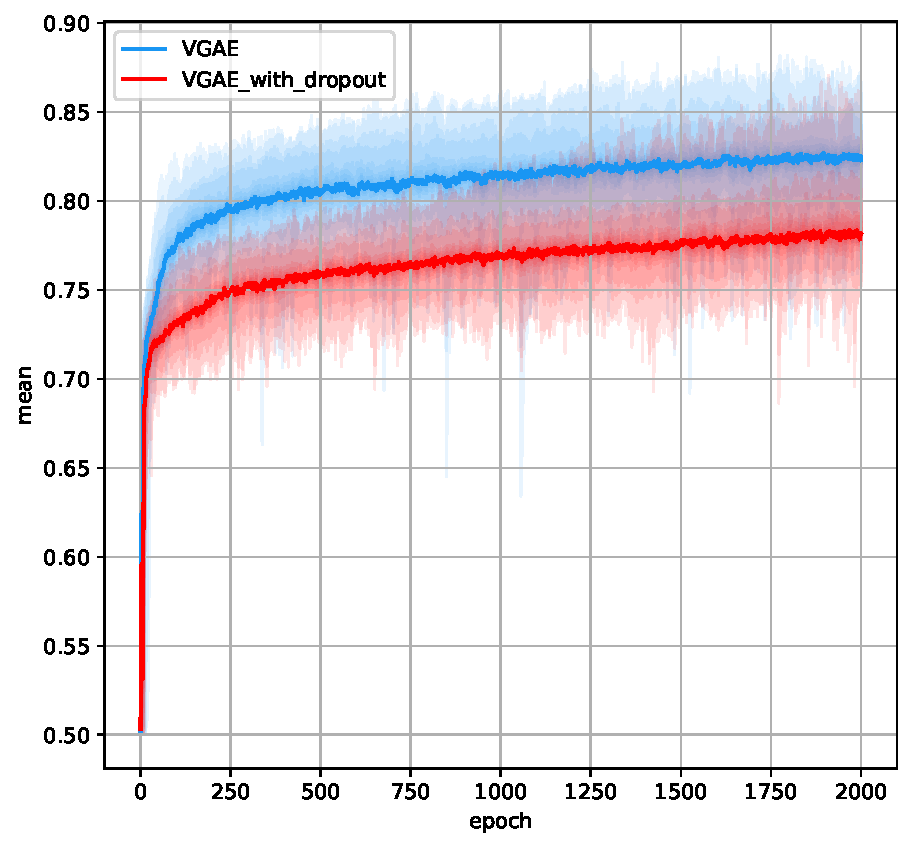
\includegraphics[width=\textwidth]{graphics/AUCs_degree_dropout_cinf.svg.pdf}
      \centering
      \caption{AUC ROC au cours de l'apprentissage\\ avec l'information de degrée}
    \end{subfigure}
    \begin{subfigure}{0.45\textwidth}
      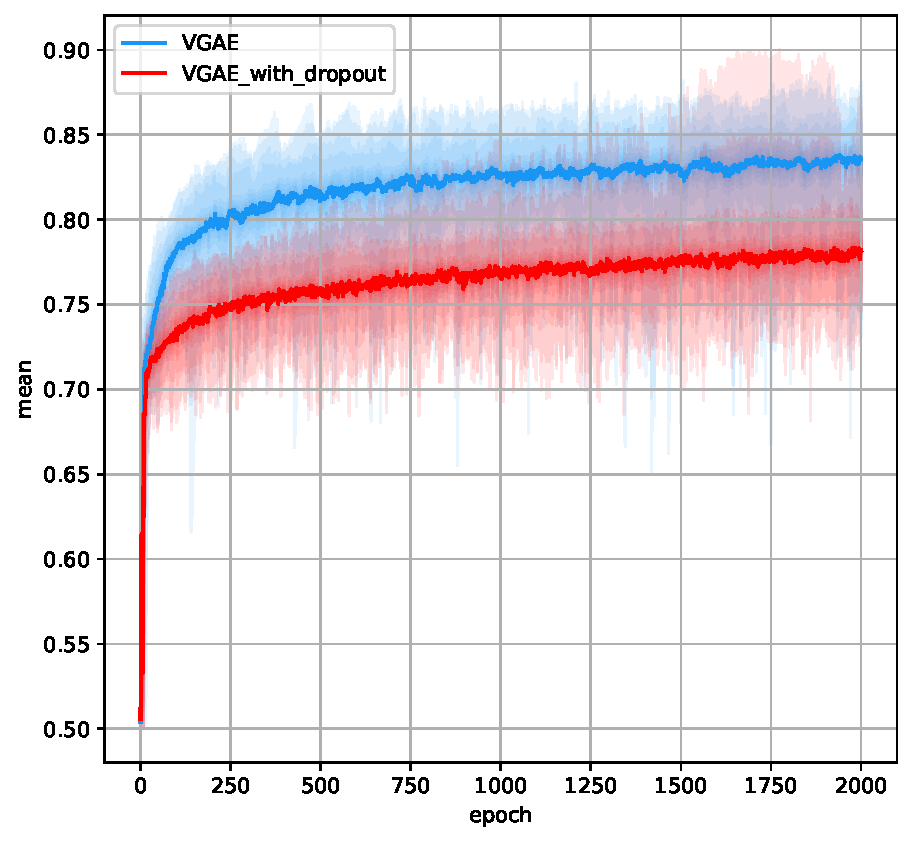
\includegraphics[width=\textwidth]{graphics/AUCs_no_degree_dropout_cinf.svg.pdf}
      \centering
      \caption{AUC ROC au cours de l'apprentissage\\ sans l'information de degrée}
    \end{subfigure}
    \caption{Évolution de l'AUC et de la précision moyenne au cours de l'apprentissage dans les deux cas (degrée connu ou inconnu)}
    \label{fig:dropout}
\end{figure}

\section{Performance de décodeur}
\subsection{Méthode}
Pour améliorer le VGAE nous avons décidé d'entrainer en plus de l'encodeur un décodeur. 
Le décodeur que nous avons entrainé est constitué de deux couches linéaire.
La fonction d'activation entre les deux couches est ReLu.
En sortie du décodeur la fonction d'activation est une sigmoîde
Les modèles ont été entraîné sur 2000 epochs. 
Ce processus a été répété 60 fois pour obtenir des statistiques sur l'apprentissage.
Le processus a été réalisé à la fois dans la situation ou le degré est inconnu et dans la situation ou il est connu.

\subsection{Performance}


\begin{table}[H]
    \centering
    \begin{tabular}{|c|c|c|}
        \hline
        Modèle & AUC & AP\\
        \hline
        GAE & 0.72 & 0.64\\
        \hline
        GAE avec décodeur & 0.94 & 0.93\\
        \hline
        VGAE & 0.83 & 0.75\\
        \hline
        VGAE avec décodeur & 0.97 & 0.96\\
        \hline
    \end{tabular}
    \caption{Performance du décodeur en moyenne sur 10 au bout de 1000 époques. voir figure \ref{fig:fig_AUC} et \ref{fig:fig_AP}}
    \label{tab:performance_decodeur}
\end{table}

\subsection{Performance avec le degré}

\begin{table}[H]
    \centering
    \begin{tabular}{|c|c|c|}
        \hline
        Modèle & AUC & AP\\
        \hline
        GAE & 0.74 & 0.66\\
        \hline
        GAE avec décodeur & 0.97 & 0.97\\
        \hline
        VGAE & 0.78 & 0.70\\
        \hline
        VGAE avec décodeur & 0.97 & 0.96\\
        \hline
    \end{tabular}
    \caption{Performance du décodeur en moyenne sur 10 au bout de 1000 époques avec le degré de chaque nœud. voir figure\ref{fig:fig_AUC_avec_degre} et \ref{fig:fig_AP_avec_degre}}
    \label{tab:performance_decodeur_avec_degre}
\end{table}

\section{Reconstruction de graphe}
\subsection{Méthode}
Nous avons choisi de tester nos modèles d'une manière plus visuelle, en cherchant à reconstruire un graphique représentant les liaisons aériennes entre les différents aéroports de notre ensemble de données. Pour ce faire, nous avons suivi une préparation des données similaire à celle décrite dans la section précédente. Nous avons ensuite entraîné nos modèles en utilisant une base de liens positifs pour l'entraînement. Par la suite, nous avons généré des graphiques en encodant les mêmes liens positifs et en décodant un ensemble de liens provenant de l'ensemble de données d'origine, ainsi qu'un nombre équivalent de liens négatifs. Nous avons ensuite enregistré plusieurs métriques, notamment le nombre de liens correctement prédits, le nombre de liens faussement prédits (qui n'existent pas dans nos données), le nombre de liens manqués (qui existent dans nos données mais ont été rejetés par le modèle), et le nombre total de liens rejetés.
Nous avons utilisés 4 modèles :
\begin{itemize}
    \item un GAE avec un encodeur formé d’une seule couche de convolution.
    \item un VGAE sans notre décodeur.
    \item un VGAE avec notre décodeur.
    \item un même GAE mais avec notre décodeur.
\end{itemize}

Chaque modèle a été testé sur un total de 27 093 liens possibles, comprenant 13 547 liens positifs et 13 546 liens négatifs. L'objectif était de couper ce jeu de liens en deux en conservant les liens les plus plausibles pour le modèle. Pour ce faire, chaque modèle attribue un score entre 0 et 1 à chacun des 27 093 liens. Ensuite, à l'aide de la méthode \texttt{torch.quantile(z, 0.5)}, nous déterminons un seuil de score pour ne conserver que les 13 546 ± 1 liens ayant un score supérieur au seuil. Ce sont ces liens qui seront considérés comme prédis positivement par le modèle. Dans nos résultats, les pourcentages associés aux liens corrects et faux sont basés sur le nombre de liens considérés positifs par le modèle (Corrects + Faux) et le pourcentage de liens manqués par rapport au total de liens positifs réels (13 547).
La prédiction est faite sur les données de \textbf{latitude}, \textbf{longitude},  et \textbf{pays} de chaque nœud.\newline
\newline
Les liens en noir sont les liens correctement prédis.\newline
Les liens en rouge sont les liens faussement prédis.\newline
Les liens en vert sont les liens manqués.

\subsection{Résultats}

\begin{table}[H]
    \centering
    \begin{tabular}{|c|c|c|c|c|c|}
        \hline
        Modèle & Min & Max & Moyenne & Écart type & Seuil\\
        \hline
        GAE & 0 & 1 & 0.75929 & 0.42746 & 1\\
        VGAE & 0 & 1 & 0.71422 & 0.45044 & 1\\
        GAE avec décodeur & 0 & 0.99980 & 0.49157 & 0.39727 & 0.54739\\
        VGAE avec décodeur & 0 & 1 & 0.56486 & 0.42113 & 0.75337\\
        \hline
    \end{tabular}
    \caption{Statistiques des scores établies par les modèles}
    \label{tab:statistiques_scores}
\end{table}

\begin{table}[H]
    \centering
    \begin{tabular}{|c|c|c|c|c|c|c|c|}
        \hline
        Modèle & \multicolumn{2}{c|}{Corrects} & \multicolumn{2}{c|}{Faux} & \multicolumn{2}{c|}{Manqués} & Rejetés\\
        \hline
        GAE & 13298 & 64.7\% & 7257 & 35.3\% & 249 & 1.84\% & 6538\\
        VGAE & 13381 & 71.0\% & 5473 & 29.0\% & 166 & 1.23\% & 8239\\
        GAE avec décodeur & 11804 & 87.1\% & 1743 & 12.9\% & 1743 & 12.9\% & 13546\\
        VGAE avec décodeur & 12199 & 90.0\% & 1348 & 10\% & 1348 & 10\% & 13546\\
         \hline
    \end{tabular}
    \caption{Résultats de prédictions \ref{fig:fig_graphe_GAE} \ref{fig:fig_graphe_GAE_with_decodeur} \ref{fig:fig_graphe_VGAE} \ref{fig:fig_graphe_VGAE_with_decodeur}}
    \label{tab:resultats_reconstruction}
\end{table}

Il est notable que les modèles sans décodeur ont manqué beaucoup moins de liens par rapport aux modèles avec décodeur. Cependant, cette amélioration s'accompagne d'une plus grande acceptation de faux liens qui auraient dû être rejetés. Cette tendance s'explique en partie par la manière dont ces modèles attribuent des scores, sans faire de distinction nette entre les liens potentiellement positifs et les liens considérés comme certainement positifs.

\subsection{Résultats bis}
Lors de nos tests, nous avons exploré l'incorporation des degrés de chaque nœud pour la prédiction de liens. Nous avons alors cherché à tester de manière plus visuelle nos modèles.

\begin{table}[H]
    \centering
    \begin{tabular}{|c|c|c|c|c|c|}
        \hline
        Modèle & Min & Max & Moyenne & Écart type & Seuil\\
        \hline
        GAE & 0 & 1 & 0.73815 & 0.43963 & 1\\
        VGAE & 0 & 1 & 0.75625 & 0.41074 & 1\\
        GAE avec décodeur & 0 & 1 & 0.49266 & 0.45323 & 0.5414\\
        VGAE avec décodeur & 0 & 1 & 0.51289 & 0.43108 & 0.5917\\
        \hline
    \end{tabular}
    \caption{Statistiques des scores établies par les modèles en tenant compte du degré des nœuds}
    \label{tab:statistiques_scores_avec_degre}
\end{table}

\begin{table}[H]
    \centering
    \begin{tabular}{|c|c|c|c|c|c|c|c|}
        \hline
        Modèle & \multicolumn{2}{c|}{Corrects} & \multicolumn{2}{c|}{Faux} & \multicolumn{2}{c|}{Manqués} & Rejetés\\
        \hline
        GAE & 13239 & 66.2\% & 6745 & 33.8\% & 308 & 2.27\% & 6797\\
        VGAE & 11665 & 74.5\% & 3995 & 25.5\% & 1882 & 13.9\% & 11427\\
        GAE avec décodeur & 12695 & 93.7\% & 852 & 6.3\% & 852 & 6.3\% & 12695\\
        VGAE avec décodeur & 12535 & 92.5\% & 1011 & 7.5\% & 1012 & 7.5\% & 13547\\
         \hline
    \end{tabular}
    \caption{Résultats de prédictions en tenant compte du degré des nœuds}
    \label{tab:resultats_reconstruction_avec_degre}
\end{table}

Nous pouvons constater que tous les modèles obtiennent de meilleures performances lorsque le degré des nœuds est pris en compte. Notamment, dans ce contexte, le modèle GAE avec décodeur surpasse en performance le modèle VGAE avec décodeur.



\section{Ablation study}

\section{Annexes}

\subsection{Performance}
\begin{figure}[H]
    \centering
    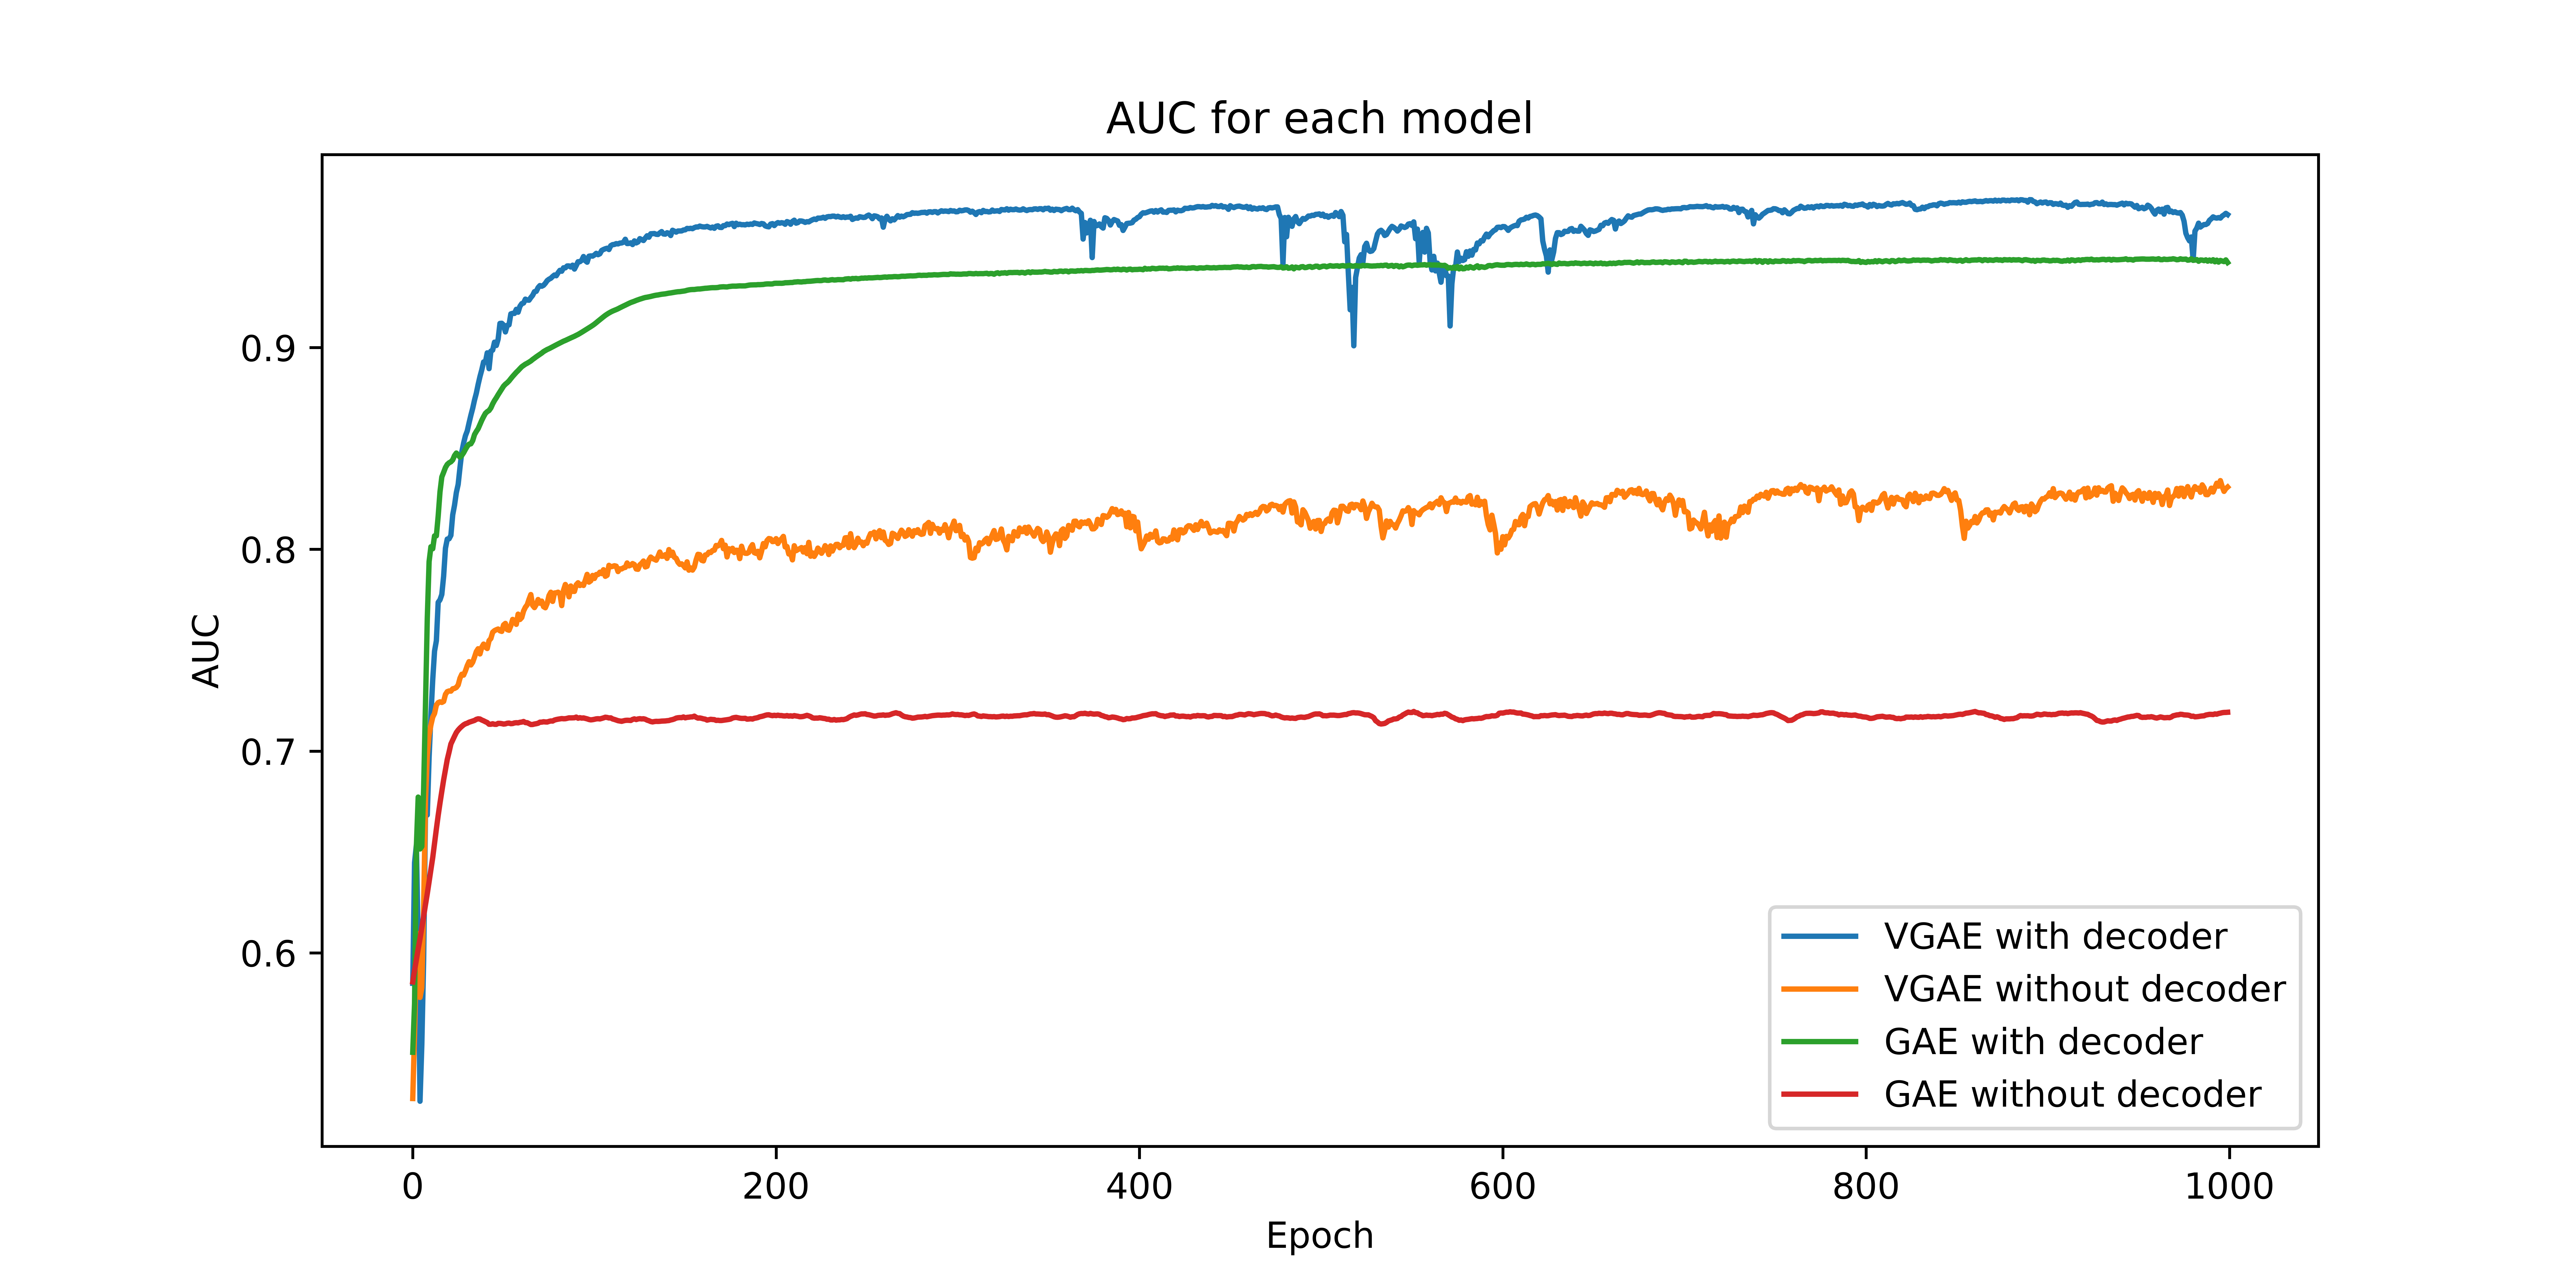
\includegraphics[width=1\linewidth]{../test_performance/sans_degre_0dropout/AUC.png}
    \caption{AUC des modèles au cours des époques}
    \label{fig:fig_AUC}
\end{figure}

\begin{figure}[H]
    \centering
    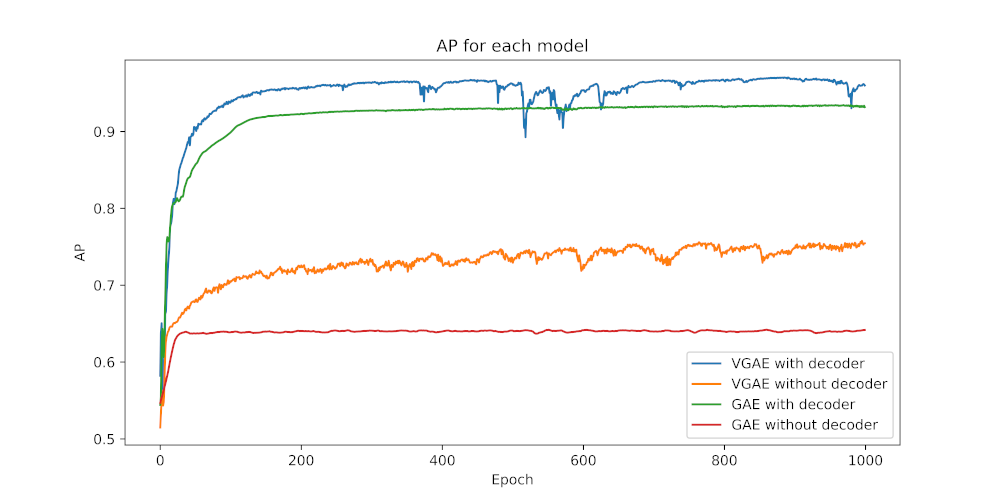
\includegraphics[width=1\linewidth]{../test_performance/sans_degre_0dropout/AP.png}
    \caption{AP des modèles au cours des époques}
    \label{fig:fig_AP}
\end{figure}

\begin{figure}[H]
    \centering
    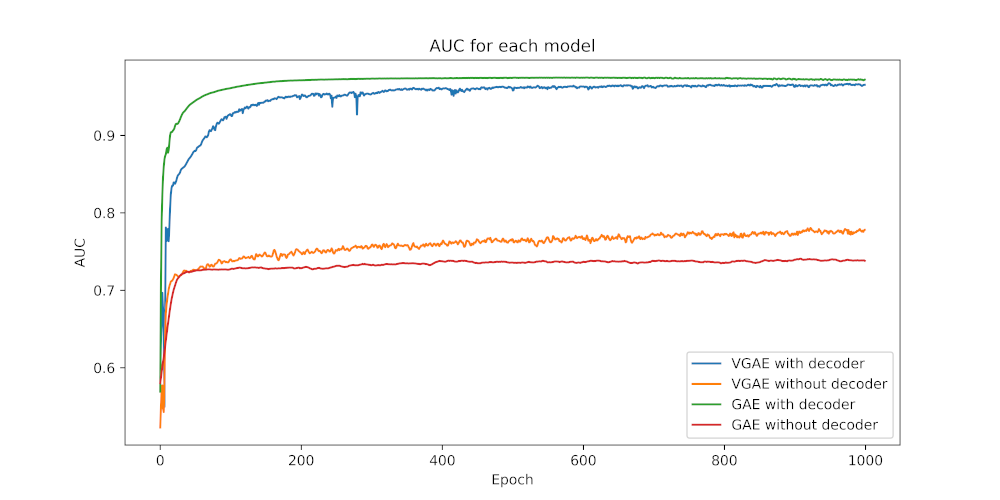
\includegraphics[width=1\linewidth]{../test_performance/avec_degre_0dropout/AUC.png}
    \caption{AUC des modèles au cours des époques en tenant compte du degré de nœuds}
    \label{fig:fig_AUC_avec_degre}
\end{figure}

\begin{figure}[H]
    \centering
    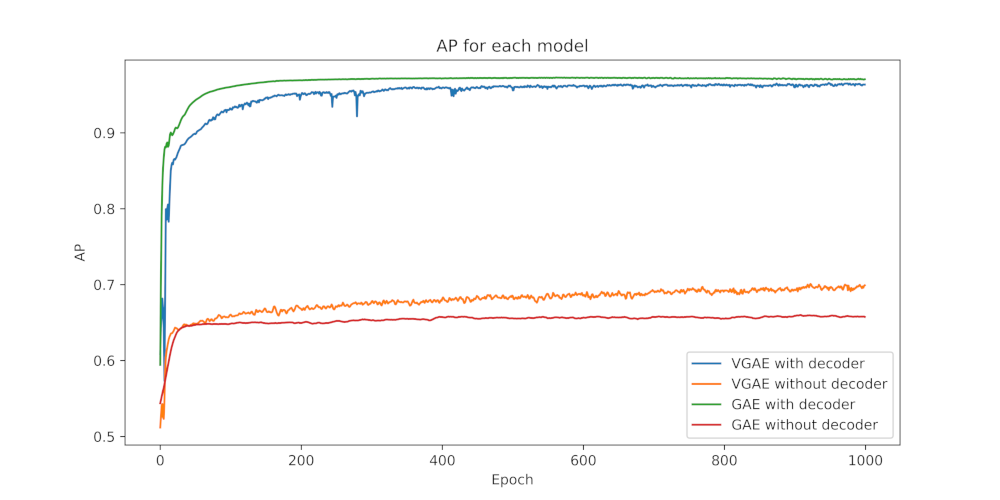
\includegraphics[width=1\linewidth]{../test_performance/avec_degre_0dropout/AP.png}
    \caption{AP des modèles au cours des époques en tenant compte du degré de nœuds}
    \label{fig:fig_AP_avec_degre}
\end{figure}

\subsection{Reconstruction de graphe}

Les liens en noir sont les liens correctement prédis.\newline
Les liens en rouge sont les liens faussement prédis.\newline
Les liens en vert sont les liens manqués.

\begin{figure}[H]
    \centering
    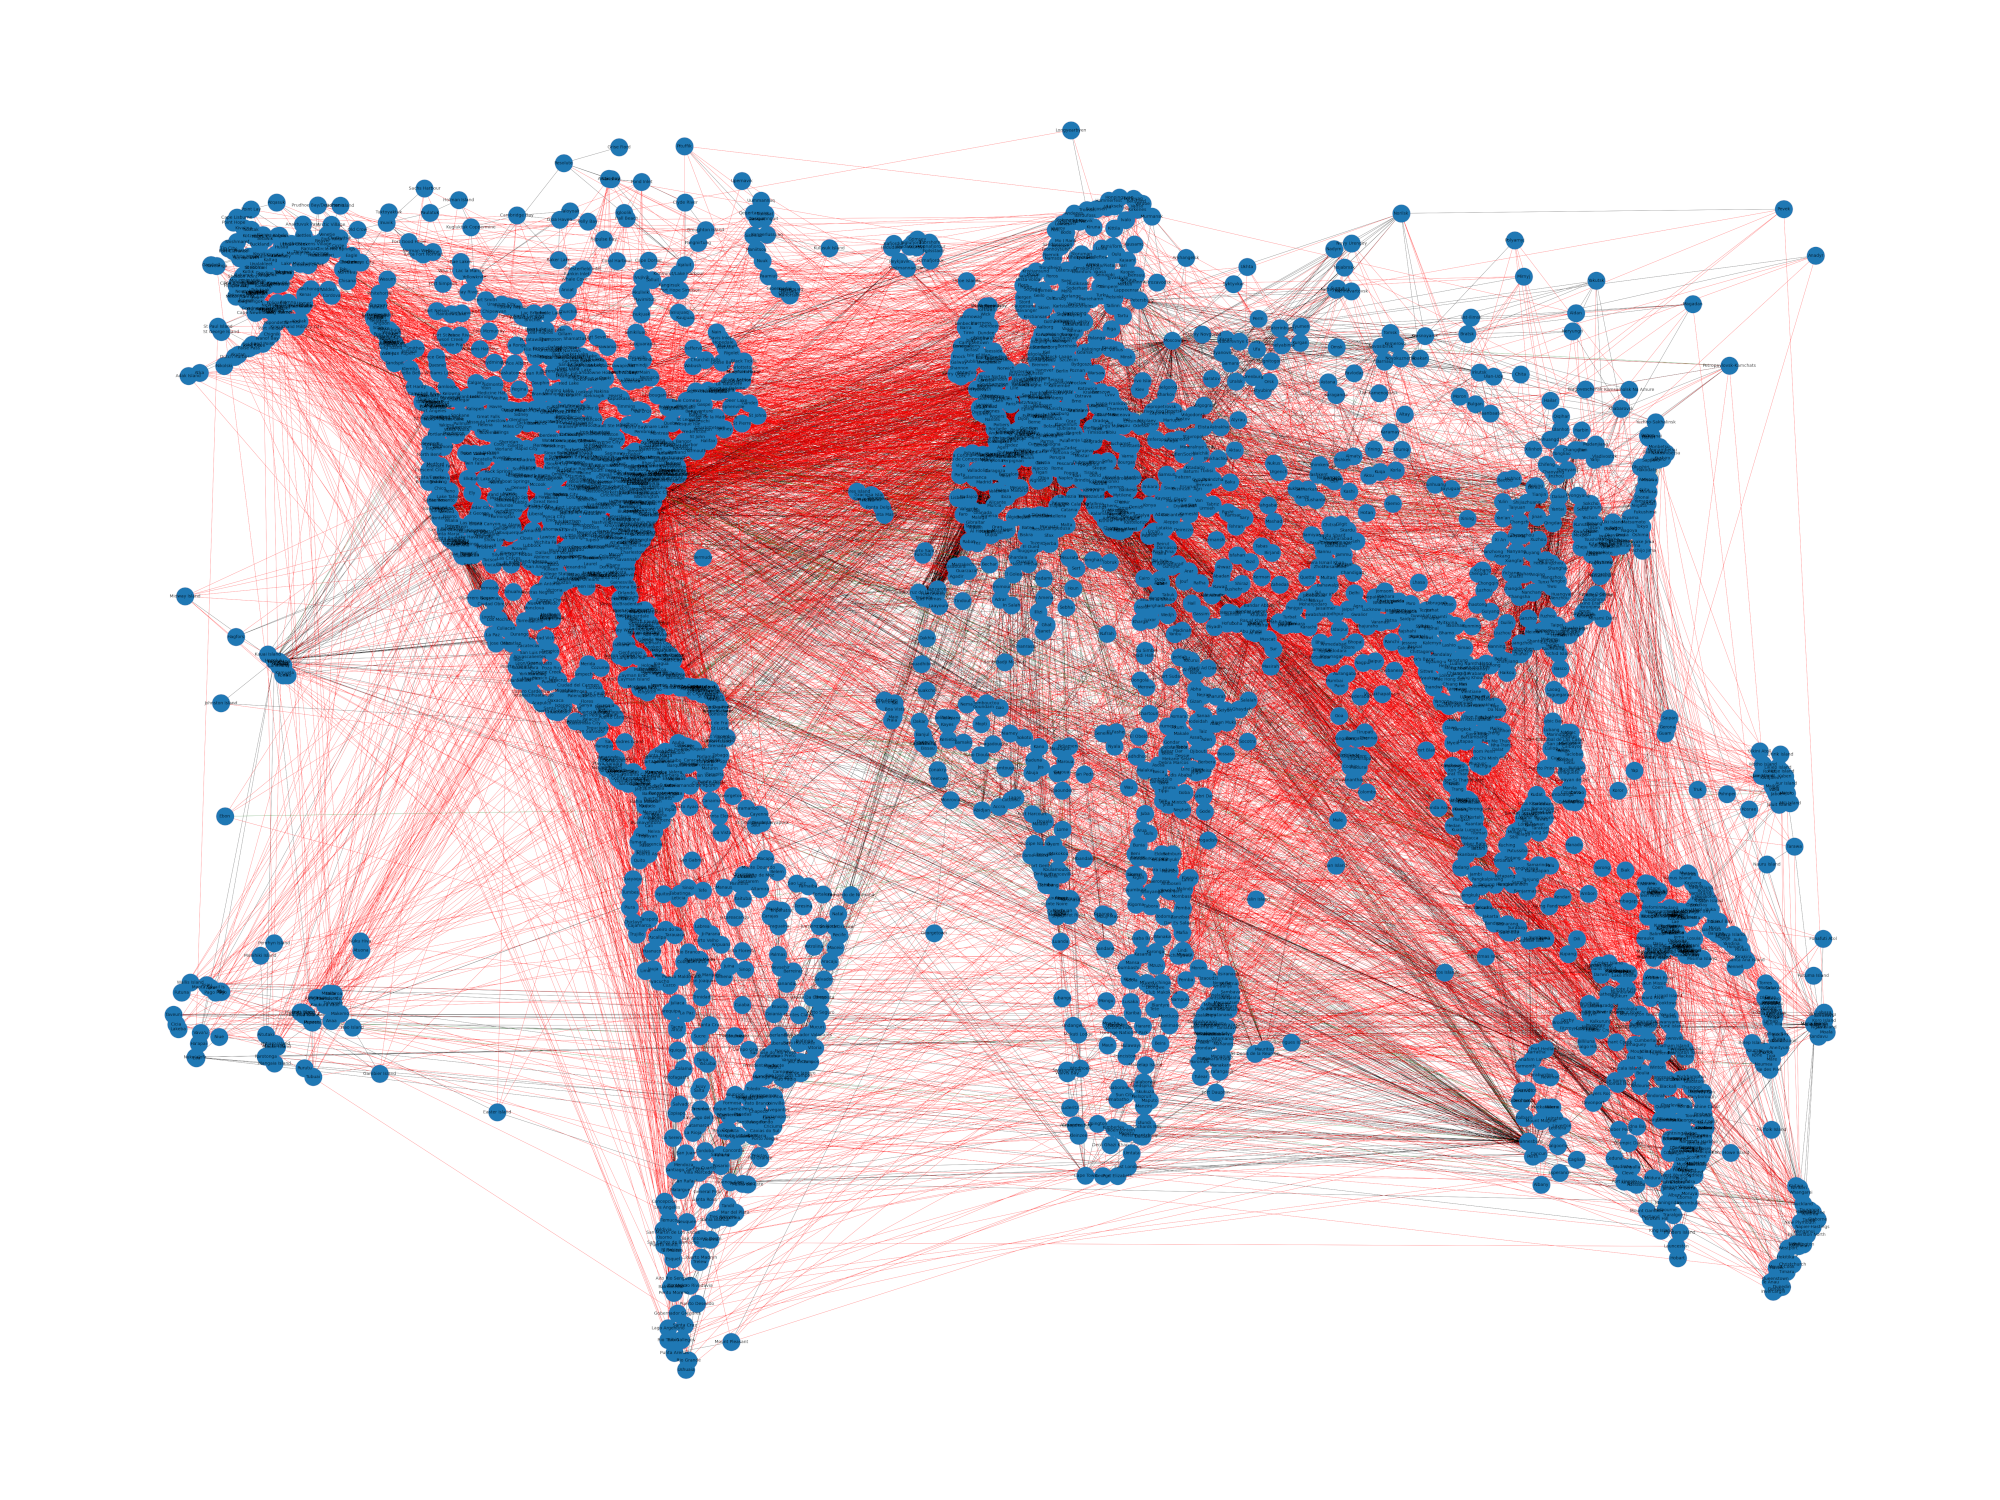
\includegraphics[width=1\linewidth]{../GCN.png}
    \caption{Reconstruction du graphe avec le GAE}
    \label{fig:fig_graphe_GAE}
\end{figure}

\begin{figure}[H]
    \centering
    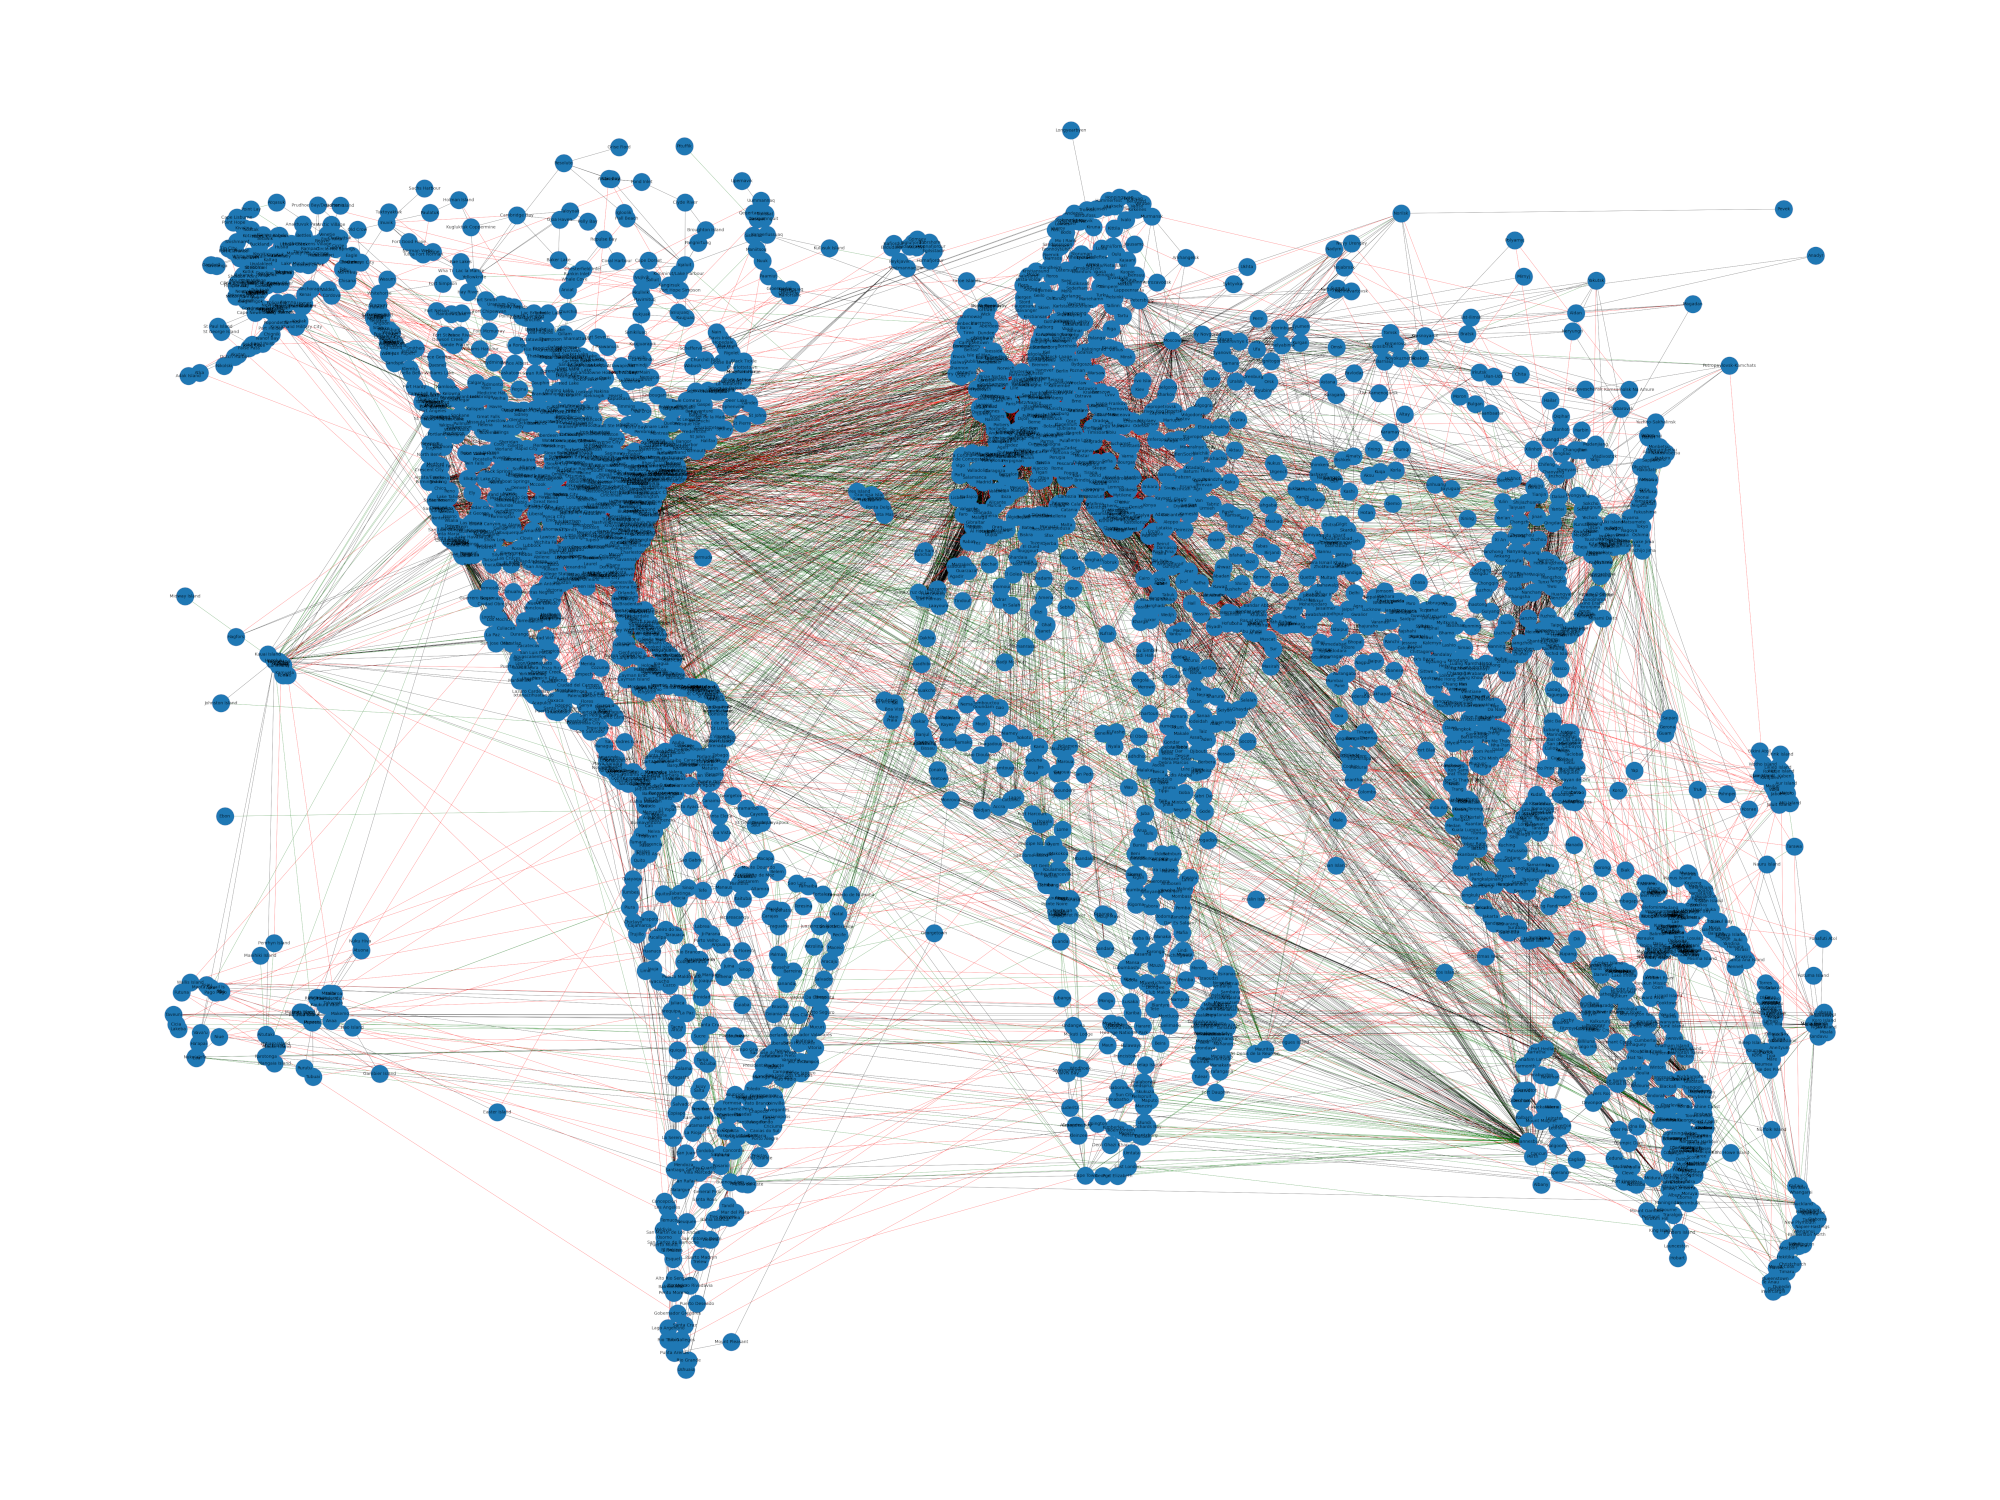
\includegraphics[width=1\linewidth]{../GCNwithDecoder.png}
    \caption{Reconstruction du graphe avec le GAE muni de notre décodeur}
    \label{fig:fig_graphe_GAE_with_decodeur}
\end{figure}

\begin{figure}[H]
    \centering
    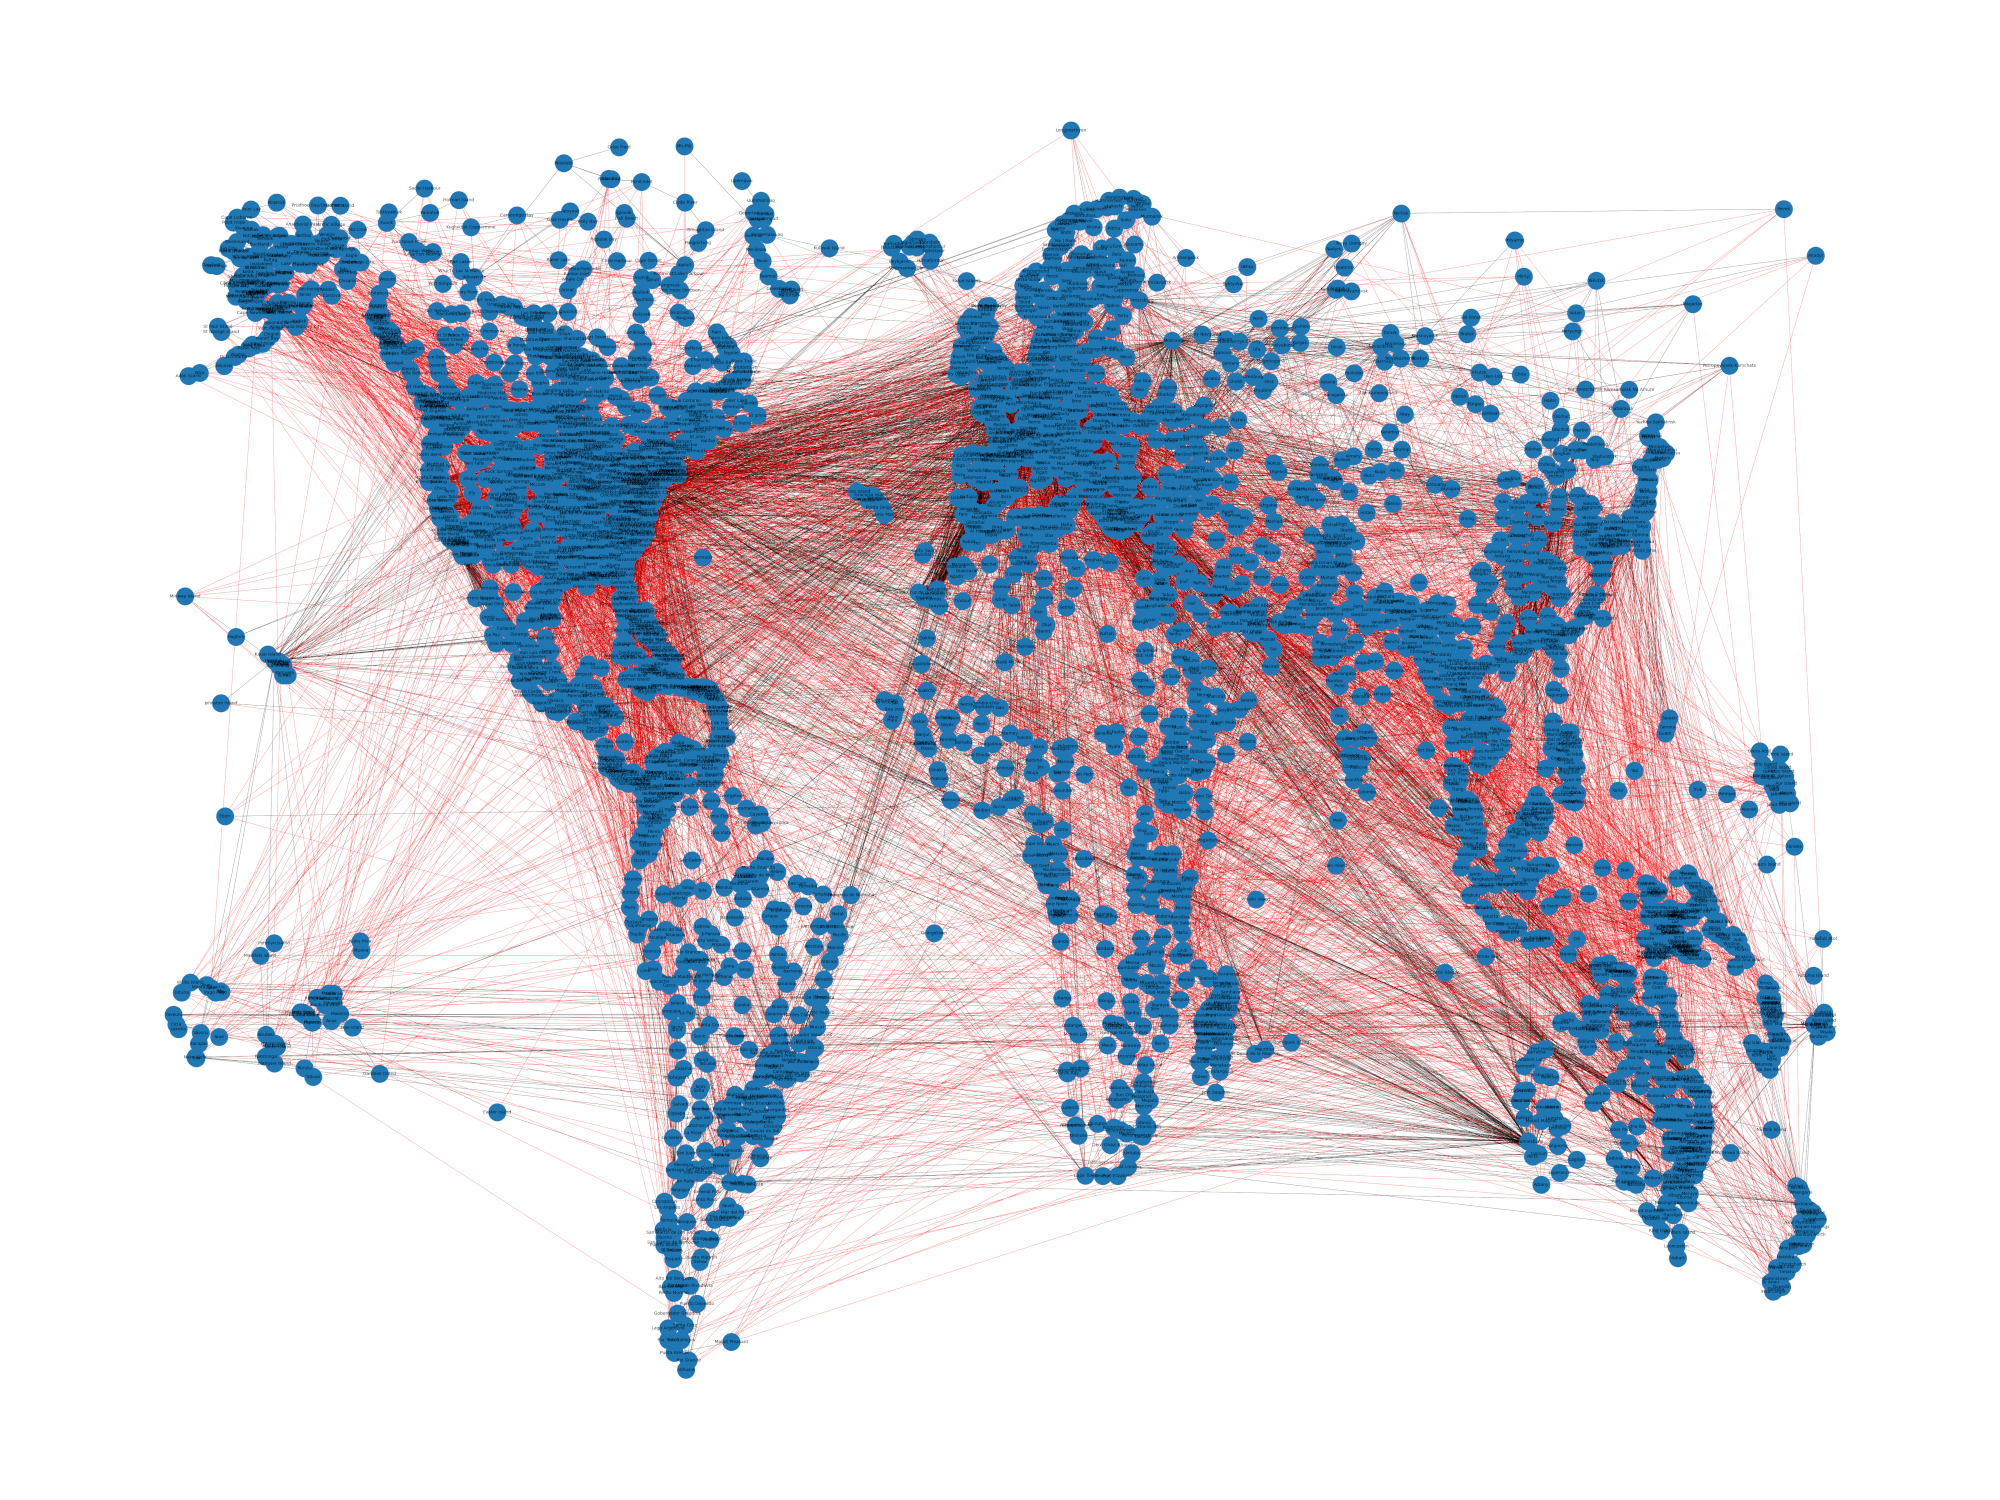
\includegraphics[width=1\linewidth]{../withoutDecoder.png}
    \caption{Reconstruction du graphe avec le VGAE}
    \label{fig:fig_graphe_VGAE}
\end{figure}

\begin{figure}[H]
    \centering
    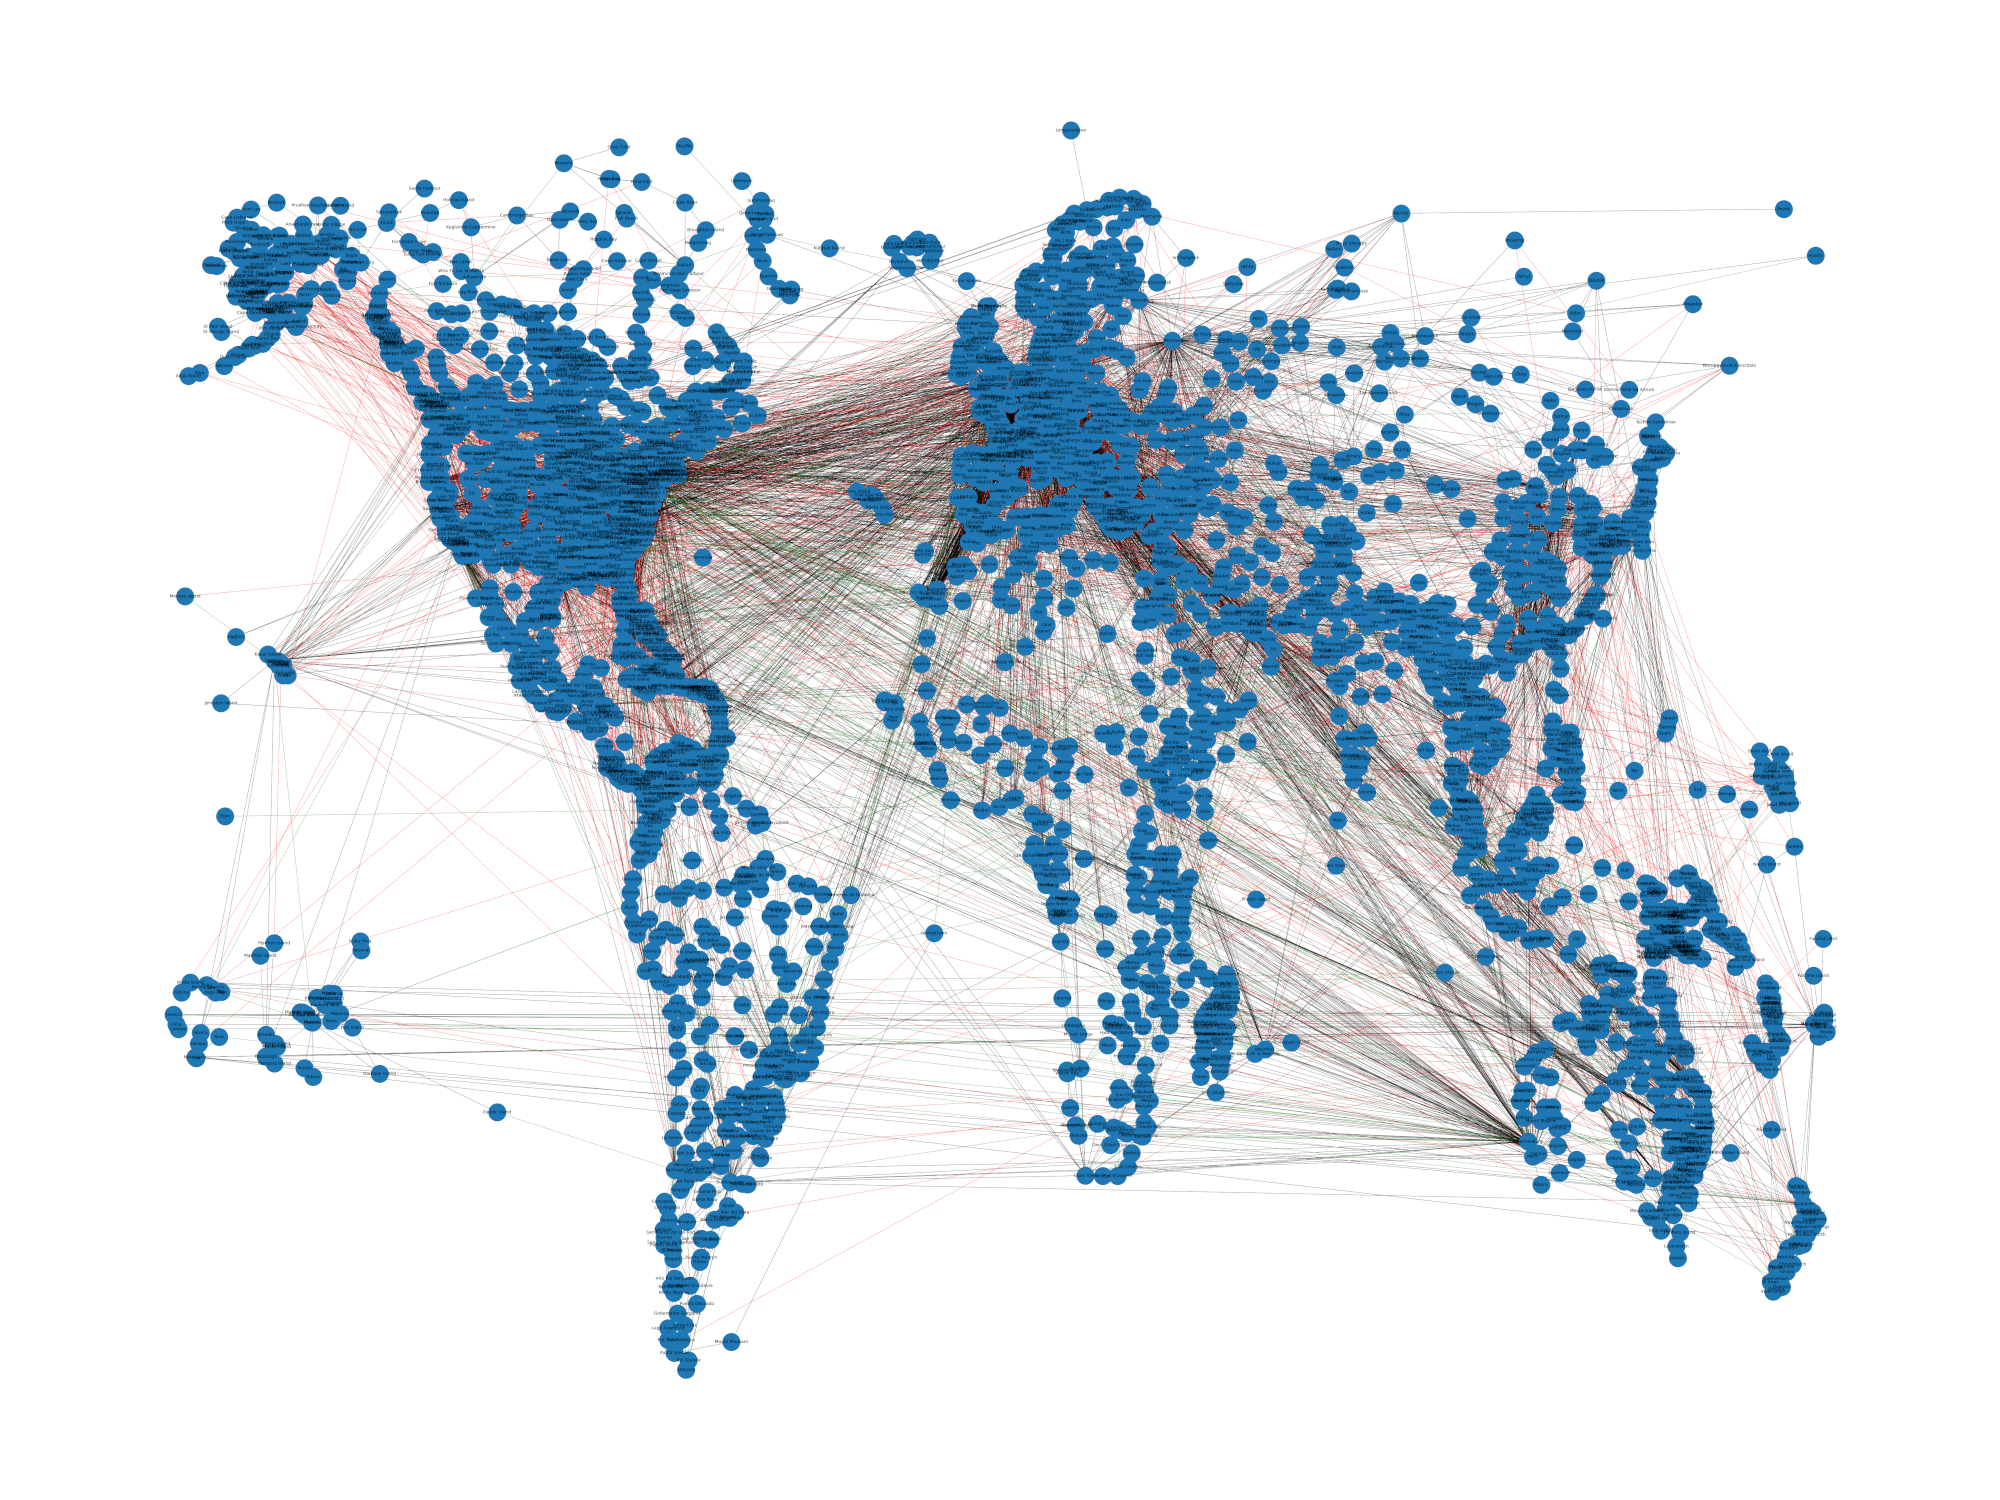
\includegraphics[width=1\linewidth]{../withDecoder.png}
    \caption{Reconstruction du graphe avec le VGAE muni de notre décodeur}
    \label{fig:fig_graphe_VGAE_with_decodeur}
\end{figure}

\end{document}
